\chapter{Research method}

\section{Terminology}\label{definitions}
The number of terms and expressions is used throughout this thesis. This chapter provides
their definitions and detailed explanations.

\textit{\textbf{Artifact}} in software engineering, is a generic term used for identification
of many kinds of software process byproducts such as specification documents, use cases, 
risk assesments, defect reports, etc. These are called byproducts because this entities
arise from the performing process itself rather than being the results produced by the process.

The subset of software process artifacts, which is particularly relevant for my thesis, 
and will be examined and used thorougly, is the set of software change artifacts - 
elctronic records which stem out of the software change processes.

\textit{\textbf{Process}} in engineering, is a term usually used for a set of interrelated 
steps which transform an input into desired output. These steps are carried out by the process
enactors: people, machines, or natural forces. 

In software engineering, the meaning of process is similar to that and used for a set of steps 
which are designed to transform some input software artifacts (the code, design documents, 
or use cases) into desired output, which can be a transformed version of input, or a
distinct product. For example, code review process is designed to transform an input - the 
source code into an output - a list of defects.

However, in this thesis, I will use perm \textit{\textbf{process}} as an umbrella term for 
larger sets of software-engineering entities which meant to impose a structure or order on
the software development activity. These entities include, but not limited to a software 
development life cycle model, software method or techniques, rules or action plans. 

\textit{\textbf{Methodology}}, according to the Oxford dictionary, is defined as a system of 
methods used in a particular area of study or activity. In context of this thesis the 
term methodology is used for a guideline system aiming on solving a problem. Usually, 
methodology consist of specific components such as tasks, methods, techniques and tools, 
and usually applied in phases. Overall methodology is not a single method, but rather 
a processes to be followed, a generic framework that can be further broken down into 
sub-processes.

\textit{\textbf{Method}}, according to the Oxford dictionary, is a particular procedure for 
accomplishing or approaching something, especially a systematic or established one.

\textit{\textbf{Behavior}} in context of this thesis is the range of actions performed by 
individuals or a team in a response to internal or external stimuli. These stimuli can be
further classified on conscious or subconscious, and voluntary or involuntary. 

The terms process and behavior are interconnected in the context of software development
in a sense that human behaviors in software development activity thought to be largely influenced 
by software processes. Nevertheless, whether modulated by software process, or just 
performed arbitrary, activities performed within software development cycle will be called 
behaviors in the context of this thesis.

\textit{\textbf{Temporal structure}} in context of this thesis is the temporal pattern of
a single activity or a set of activities performed by individual or a group. 

\textit{\textbf{Activity cycle}}, or \textit{\textbf{temporal container}} in context of 
this thesis is an abstraction of temporal window containing temporal structure (structures).

\section{Software processes}\label{software.processes}
There are different approaches for software development which were designed in order to 
facilitate the creation of software systems. These approaches provide means for 
structuring of development activity. The main goal of imposing such a structure on the 
development process is to organize production of code in manageable way. 
According to the research, structuring software process yields a number of benefits:
\begin{itemize}
 \item whole software development cycle can be broken down onto number of one-step pieces;
 \item which, in turn, helps to keep clear focus on what must be delivered and when, during each step;
 \item it clarifies the project scope and improves time, effort, and cost estimates;
 \item it provides ability to measure the progress;
\end{itemize}
It is strongly advocated, that the use of established and well structured process is 
essential for the complex projects in order to orchestrate collaborative effort 
of multiple teams. 

\subsection{Software process models}
Structuring software development includes the use of a software process model and following 
a software method, known as methodology. While latter is used primarily to navigate 
through the development process: determining a number of functional points, 
designing data flow diagrams, etc., the model provides developers with guidance about their 
tasks and the software development activities that should be undertaken. 
This definition of steps and ordering of carried activities facilitates
a framework for estimation of resources, defines major milestones, and provides 
means for time and effort monitoring and management. 

All of software process models include three generic steps, or high-level phases, 
corresponding to software life cycle: definition phase, development phase, and a maintenance phase. 
The definition phase includes the initial planning of the future system and 
the requirements collection: developers identify data need to be processed by the system, 
its functionality, behavior, and what constraints must be placed on the system design 
and development. 
The development phase focuses on the system implementation and testing: 
developers write the system code, test if the system satisfies to user requirements, 
has planned behavior, and produces needed output. 
The last, maintenance phase, focuses on the post-development activities: 
system deployment and its operational support. 

In each software model these large phases are composed of series of smaller, distinct phases.
Each of these phases is executed with a particular 
goal: some will provide a part of the software system, or perform its validation, 
while other will deliver the engineering documentation, or a user manual. 
Examples of such phases are the requirements collection, user manual writing, 
coding of a a functional module, etc.
The determination of these small phases, its ordering, and the definition of the phase-transitioning 
criteria are different from model to model.

\fxnote{should I put examples of models to here, their key advantages and disadvantages?}

\subsection{Software process modeling research}
The research area dealing with Software Process Modeling (SPM) was receiving significant 
attention over the years and is recognized as one of the powerful technologies
in software process engineering. The empirical approach techniques play a critical role
in SPM and most of the work is based on the case studies and action research. 
However, this approach has an intrinsic flaw - it is hardly feasible since
empirical SPM research activities are limited by organizational context, and also extremely 
expensive - some of the known reports required decades to obtain an empirical evidence.
Thus, in most cases, it is unfeasible to perform an explanatory research in full rigor,
and as pointed in \cite{citeulike:11079867}: ``Currently the empirical studies in SPM were 
mostly exploratory in nature, whose strengths of empirical evidence were relatively weak...''
\fxnote{process modeling built up-down and it is expensive!}

\subsection{Software process elicitation and conformance}
Another area of research related to my work is the area of the software process conformance. 
the research in this area is dealing with methods and theories for formulating, identifying and
investigating violations in the execution of software processes. These methods heavily rely
on the process elicitation step which is of most interest \fxnote{very similar
Paragraph about ``classical'' software process research - heavyweight, expensive
mostly top-down oriented: first designed, secondly tested or confirmed}.

\section{Open Source Software processes}\label{oss.processes}
In recent time we have seen the rise of alternative software development practices. 
With development of communication technologies, groups of people were 
enabled to collaborate together over the Internet in order to create software that is 
licensed openly promoting software reuse, modification, and distribution. While there are 
hundreds of thousands of open source projects, they rarely provide any explicit details on 
their software processes, moreover, they often refuse to provide any of 
specifications \cite{Torvalds:2005}. 

From little which is known about OSS processes, they are quite different from what is 
commonly thought in the classrooms or what industrial standards tell us.

\subsection{Death of distance and cyberspace}
With the development of internet infrastructure connecting continents with ``information
superhighways'', the term ``cyberspace'', once a buzzword \cite{citeulike:11095763}, become 
a term which explicitly refer to the real-world phenomena providing an information-exchange
and collaborative medium. Unlike traditional physical space and transportation networks, where 
materials and workers are transported at limited speeds in space and time, the information 
superhighways in cyberspace form networks for digital information to be transported almost instantly 
between sites any time and at almost any place. 
Novel communication and collaboration techniques such as videoconferencing and software change 
control systems offer developers great flexibility to control their interaction and collaboration. 
It is possible to interact synchronously or asynchronously from any location and at any time. 
Once software project and developers are online, in cyberspace, not only geographic measures, but 
any geographic notions that are based on the principle of distance friction, such as distance decay,
are not longer applicable to participants and to the software product.

\subsection{Relaxation of space-time constraints, extensibility and displacement}
Time and space constraints significantly influence and shape human activities. There are 
particular research areas dedicated to study the effect of these constraints on individuals 
and society. For example the Hägerstrand's time geography in the Regional science and is 
a powerful conceptual framework which integrates the temporal and spatial dimensions of
human activity patterns. It conceives and represents an individual’s activities and travel 
in a 24-hour day as a continuous temporal sequence in geographical space. The trajectory 
traces this activity sequence as a space-time path in a 3D space-time container composed by a
geographic plane and a Z-axis representing a time dimension. Using this framework, researchers
build space-time paths, illustrating how a person navigates through a spatial-temporal environment.
Using this framework, Hägerstrand demonstrated that human spatial activities are often governed by
three types of constraints: capability, coupling, and authority. Here, the capability constraints
refer to the limitations on human movements due to physical or biological factors, for
example, a person cannot be in two places at one time, but not anymore - however cyberspace allows 
one to actually be present in two places virtually - two chat rooms, or video-conferences.
A coupling constraint refers to the need to be in one particular place for a given length of time 
to be in interaction with other people, not anymore again, high frequency asynchronous
information exchange allows one not only to be ``coupled'' to multiple people, but to multiple 
people in multiple places. And the third constraints, an authority constraint refers to an 
area that is not accessible to particular individuals or groups, which is also shrinked.
\fxnote{nice explanation of how cyberspace and OSS relaxed all three}

Basically

\subsection{The Bazaar model and impact of small changes on the process visibility}
\begin{figure}[tbp]
   \centering
   \includegraphics[height=115mm]{commit-often.eps}
   \caption{Illustration of the contemporary trend advocating small commits. 
\url{http://stackoverflow.com/questions/107264/how-often-to-commit-changes-to-source-control}}
   \label{fig:commit-often}
\end{figure}
